\documentclass{article}

% Layout
\usepackage[a4paper,margin=2.5cm]{geometry}
\parindent=0pt
\frenchspacing

% Packages
\usepackage[none]{hyphenat}
\usepackage[english]{babel}
\usepackage{parskip}
\usepackage{hyperref}
\usepackage{csquotes}
\usepackage[backend=bibtex, sorting=none, dateabbrev=false, urldate=long, maxbibnames=2]{biblatex}
\usepackage{booktabs}
\usepackage{graphicx}
\usepackage{enumitem}
\usepackage{caption}
\usepackage{subcaption}

% Bibliography configuration
\DeclareFieldFormat[article, inproceedings, online, techreport]{title}{\emph{#1}}
\DeclareFieldFormat{titlecase}{\MakeSentenceCase{#1}}
\DefineBibliographyStrings{english}{%
  techreport = {Technical report},
}
\bibliography{Report.bib}

% Hyperlink configuration
\hypersetup{colorlinks,linkcolor=black,citecolor=black,filecolor=black,urlcolor=black}

% Verbatim configuration
\makeatletter
\let \@sverbatim \@verbatim
\def \@verbatim {\@sverbatim \verbatimplus}
{\catcode`'=13 \gdef \verbatimplus{\catcode`'=13 \chardef '=13 }}
\makeatother

% Itemize configuration
\setlist[itemize,1]{leftmargin=\dimexpr 14pt}

% Document contents
\begin{document}

\title{Distributed sentiment analysis on GitHub commit comments}
\author{Leon Helwerda (s1034375) and Tim van der Meij (s1115731)}
\date{\today}
\maketitle

\begin{abstract}
  In this report we discuss performing sentiment analysis on GitHub commit
  comments. We describe the problems and solutions related to downloading and
  preprocessing the dataset and gaining insights into the data using a naive
  implementation that uses lists with positive and negative words. After
  manually labeling 2000~training examples, we benchmark several classification
  algorithms and we use the most promising classifier in our final
  implementation where we apply the trained classifier on the entire dataset.
  We visualize the overall sentiment per programming language to show the
  potential of our approach. Distributing workload is key when working with 
  such a large dataset. Therefore, getting the data, preprocessing it and 
  performing the sentiment analysis is all done in a distributed manner with 
  help of OpenMPI and MapReduce.
\end{abstract}

\section{Introduction}\label{sec:introduction}
Sentiment analysis is a technique that aims to extract subjective information
from text, audio or other multimedia. This information contains, but is not
limited to, judgements or emotions on a certain topic. Sentiment analysis is
often troubled by the limitations of natural language processing and by the
large amounts of data available. Furthermore, in order to process all samples 
from a given dataset, we require that the sentiment analysis on one sample must 
be fast. Otherwise, the process quickly becomes infeasible and unsuitable for a
huge dataset.

In this report we focus only on sentiment analysis of textual content. We 
specifically use the GitHub commit comments dataset for our analysis. GitHub is 
an online platform that provides source code hosting and collaboration for both 
open-source and closed-source projects that use the Git version control system. 
When developing source code in a version-controlled environment, it is common 
practice to divide the implementation of functionality into \emph{commits}, 
which are small packages of code. Once the developer is ready to have the code 
reviewed, then reviewers can look at these commits and comment on them. For 
instance, a reviewer could add a comment to a specific line of code and suggest 
an improvement.

The GitHub commit comments dataset that we use consists of exactly these 
comments. The commit comments are particularly interesting, since developers 
and reviewers tend to put a lot of personal feelings in them. These emotions 
can range from happiness, when a commit is of high quality, to sadness or 
angriness when a commit is of poor quality.

We perform the sentiment analysis in a distributed manner. Since the total 
GitHub commit comments dataset is very large, and speed and efficiency are 
a concern, we aim to distribute most of the workload, including downloading and 
preprocessing data, over several worker nodes. We first implement a naive 
algorithm to get insights into the dataset and then apply those insights to the 
final implementation that uses a classifier to quickly classify commit comments 
as being positive, negative or neutral. Furthermore, we link the commit 
comments to the main programming language used in the code repository to be 
able to get insights into the sentiments of the developers per language.

Section~\ref{sec:problem} describes the research question in more detail as well
as give definitions of the techniques that we evaluate and related work. The
used dataset and the implementation of the distributed sentiment analysis
framework are discussed in Section~\ref{sec:dataset} and
Section~\ref{sec:implementation}, respectively. We present our experiments and
results in Section~\ref{sec:experiments-and-results}. We list future research
and conclude our analysis in Section~\ref{sec:conclusion}.

\section{Problem statement}\label{sec:problem}
The goal of this research is to determine how we can perform sentiment analysis
on a large dataset in a distributed manner. In order to investigate this, we
develop a complete sentiment analysis framework in Python that contains all
techniques discussed in this report. The implementation is further outlined in 
Section~\ref{sec:implementation}.

Sentiment analysis allows for the retrieval of subjective information, such as
opinions, judgements or emotions, from text or other multimedia. Several types
of sentiment analysis exist, but the most used are classification of content
into an emotion category (`happy', `angry', `disappointed', et cetera) or
classification of content as being positive, negative or neutral. Since
sentiment analysis through the use of classification yields a probability score
for all categories, we are also able to numerically compare the sentiment in
different content, making it possible to determine if one piece of text is more
positive than another, for example. Our research focusses on performing 
sentiment analysis on textual content and classifying the textual content as 
being positive, negative or neutral.

Being able to automatically classify content into fixed categories can yield
previously unknown insights. Because of this, sentiment analysis is becoming
increasingly important for companies all over the world that want to know how
users review their products or services. For instance, web shops like Amazon
are interested in determining which products reviewers are positive about.
With this information Amazon might decide to recommend those products over
products with less positive reviews, thereby increasing customer satisfaction
and revenues. Users on a discussion platform can also benefit from sentiment 
analysis in order to detect whether a certain discussion has a positive or 
negative atmosphere.

Sentiment analysis is troubled by the limitations of natural language processing
as well as by the large amounts of available data. Natural language processing
limitations include, but are not limited to, making proper use of context and
detecting sarcasm. On top of that, sentiment analysis on a single text should be
fast in order to make working with a large dataset feasible.

% TODO: Perhaps split up in subsections?
% Perhaps also mention: "How do we obtain the dataset and preprocess it?"
% And: "How can we distribute the work onto worker nodes?" From presentation.
We propose a framework that performs sentiment analysis on large datasets in a
distributed manner. We aim to distribute most operations performed by the 
framework, such as downloading and preprocessing individual data dumps,
classification and collection of analyzable results. We utilize the resources 
of the Distributed ASCI Supercomputer~3 (DAS-3) at the LIACS institute of 
Leiden University. The DAS-3 has a total of 32~worker nodes consisting of 
commodity hardware and a number of hard drives, including a RAID configuration. 
A key feature of the framework is the distribution of workload over multiple 
worker nodes, or even over multiple processes on a single node. This provides 
a great speed-up when processing the large datasets that we use, of which more 
details are given in Section~\ref{sec:dataset}.

We implement two different approaches for performing sentiment analysis. The
first approach is the word list approach. Given a piece of text, we split the 
text into individual words and for each word we test if the word appears in 
fixed lists of positive and negative words. We count the number of positive and 
negative words in the text and perform a majority vote for the final 
classification of positive, negative or neutral. This is a basic approach that 
is expected to perform reasonably well, but at the same time we foresee issues 
with this approach.

For instance, when this naive analyzer encounters the word `good', the 
algorithm treats that word as positive, but if that word is preceded by the 
word `not', then the meaning is actually negative. The algorithm, because of 
its simplicity, is not able to distinguish these cases, and may end up deciding 
that the text is neutral. This shows the main problem of this approach: because 
we only look at individual words, we omit the context in which these words 
appear.

To overcome these issues and to actually take context into account, we implement
a second approach that uses a classifier to do the classification. With this
approach we do not need any fixed word lists. The classifier learns what
positive, negative and neutral texts are from training examples. There are two
main difficulties for this approach, namely that there is no labeled training
set available for the dataset we use. Secondly, it is not clear which 
classifier would be the best fit for the data. We therefore start by manually 
labeling 2000~commit comments as positive, negative or neutral.

Once we have a training set, we can train many different classifiers, such as 
a random forest classifier or a Gaussian naive Bayes classifier, and perform 
five-fold cross-validation. The resulting accuracies from the cross-validation 
allow us to get an idea of which classifier is the best fit for the data. After 
having trained the best classifier with the training set, we treat the data 
that has not been used for the training set as the test set. We provide the 
test set to the classifier and let the classifier put positive, negative or 
neutral labels on the commit comments based on learned information from the 
training phase.

In order to show the potential of the latter approach, we supplement each 
commit comment with the main programming language of the repository it belongs 
to. We perform sentiment analysis on the test data and with the resulting 
labels for each commit comment we visualize the distribution of positive and 
negative commit comments per programming language. This is done in order to 
obtain insight into the sentiment of developers that use different programming 
languages. It is not hard to imagine that the results of sentiment analysis on 
this dataset can be used to obtain many more interesting insights.

\subsection{Related work}\label{sec:related-work}
There are many papers and studies related to sentiment analysis, particularly 
on sentiment scores of small pieces of text. Such studies for example 
investigate the classification of sentiments of a Twitter data 
set~\cite{agarwal2011twitter,kouloumpis2011twitter}, or perform sentiment 
analysis on movie review comments~\cite{yessenov2009sentiment}. Often, the 
empirical studies provide techniques for classifying a specific corpus and 
compare these with general classifier approaches. The novel techniques generally
require a lot of tuning in order to make use of the features in the dataset as 
much as possible.

There are also studies related to sentiment analysis of the GitHub commit 
comments dataset, which we use in our 
analysis~\cite{guzman2014github,pletea2014security}. Again, these studies often 
provide a specific sentiment analysis tool that uses lexical extraction based 
on heuristics. An experiment with a very large dataset and with numerous 
classifier variants is usually unavailable. There is one analysis of a large 
collection of GitHub commit messages which counts the number of messages that 
fall into one sentiment category and compares languages in this 
way~\cite{geeksta}. The downside of this approach is the use of a fixed word 
list that might not catch all messages and could incorrectly classify some 
messages as happy which are in fact not happy, for example.

\section{Dataset}\label{sec:dataset}
We use the GitHub commit comments dataset for our analysis. As described in the
introduction in Section~\ref{sec:introduction}, the GitHub commit comments
dataset contains comments that reviewers have attached to specific lines of
a Git commit or to an entire Git commit.

The dataset is provided by the GHTorrent project~\cite{gousios2013ghtorrent},
which publishes incremental and categorized dumps of data from the publicly
available GitHub API\@. We only use the commit comment dumps and the
repository dumps for our analysis, but, among others, issue comments, pull
request comments and events are also available. Every two months a new
incremental dump is published.

We focus on two types of dumps we use for our analysis, which are the
commit comments and repository dumps. The former is used for the sentiment
analysis itself, while the latter is used to assign to a commit the main 
programming language of the repository that it belongs to, which is useful for 
one of the experiments described in Section~\ref{sec:experiments-and-results}.

Each dump contains a part of the dataset, since GHTorrent generates incremental 
dumps on a bimonthly basis. A dump consists of one BSON file, which is 
a binary-encoded JSON file that is used for storing and exchanging data in 
a structured manner. The BSON file is converted to JSON and preprocessed, after 
which we obtain a file containing objects of the following form:

\begin{verbatim}
{
  "id": 8771097,
  "body": "It seems e.offsetX is not the way to get the relative cursor position
           in Firefox. I'm getting `undefined' in my experiments there.",
  "url": "https://api.github.com/repos/fedwiki/wiki-plugin-method/comments/8771097"
}
\end{verbatim}

We use the {\tt id} field as a unique identifier for cross-reference and
the {\tt body} field which contains the actual commit message. For the
experiments we also use the {\tt url} field to extract the name of the
repository that the commit belongs to in order to assign the main
programming language of that repository to the commit message.

The repositories dump is very similar, however, from that dump we only
extract the {\tt full\_name} field which contains the repository name and
the {\tt language} field which contains the main programming language used
in the repository.

The characteristics of both datasets (commit comments and repositories) are
listed in Table~\ref{tab:dataset}. We list details of the 2015--01--29
commit comments dump as that dump has been used for manually labeling commit
comments to create a training set, which we discuss in
Section~\ref{sec:implementation}. Furthermore, we list details of the
2015--01--29 commit comments dump when all comments with non-Latin characters
(Chinese, Russian, et cetera) have been removed. Those comments are not
relevant for our research as we only focus on English commit comments. Finally
we list the details for all commit comment dumps and all repository dumps. In
the table, `preprocessed' indicates that we have applied our preprocessor to
remove unneeded fields for our research.

\begin{table}[h]
  \centering
  \begin{tabular}{l r l}
    \toprule
    \textbf{Dump}                           & \textbf{\# items} & \textbf{Size}                           \\
    \midrule
    2015--01--29 commit comments            & 182.282           & 43~MB compressed, 267~MB uncompressed   \\
    2015--01--29 Latin-only commit comments & 165.427           & 42~MB preprocessed                      \\
    Commit comments (17 dumps)              & 1.731.251         & 434~MB compressed                       \\
    Repositories (17 dumps)                 & 12.802.797        & 10.8~GB compressed, 1.3~GB preprocessed \\
    \bottomrule
  \end{tabular}
  \caption{Characteristics of the GitHub commit comment and repository datasets.}\label{tab:dataset}
\end{table}

\section{Implementation}\label{sec:implementation}
Our implementation consists of a number of components that can interact with 
each other. Among others, we have implemented a preprocessor component for 
extracting the datasets described in Section~\ref{sec:dataset}, an analyzer and 
classifier that can generate predictions for sentiment scores, a plotting 
framework, an experiment runner and an interactive dataset labeler.

We implemented these tools using the Python programming language with 
distributed processing in mind. The components for making predictions and 
counting frequencies can be automatically distributed using MapReduce and the 
preprocessor and some parts of the toolchain can be parallelized using MPI, as 
described in more detail in Section~\ref{sec:mpi}.

Many parts of the toolchain use the notion of \emph{groups} in order to make 
analysis possible for different goals. For example, one can group the commit 
comments on their {\tt id}, which allows for visual output of the predictions 
and cross-referencing the results. The use of the {\tt score} group allows the 
reducer in Section~\ref{sec:reducer} to count the frequencies of each score, 
which can then be visualized with a frequency plot. Other groups function more 
like creating partitions of the dataset. The groups play an important role in
the filtering phase of the preprocessor from Section~\ref{sec:preprocessor},
and the plotter can also create different plots for groups, such as the
{\tt algo} group for the results of the experiment runner in
Section~\ref{sec:experiment-runner}.

\subsection{Preprocessor}\label{sec:preprocessor}
The preprocessor is the first step in the implementation. The dataset from 
Section~\ref{sec:dataset} consists of different types of dumps and is split 
into multiple incremental dumps that are generated bimonthly. Therefore, we 
need a tool to automatically perform the phases of downloading, extracting, 
converting, processing and filtering the dumps of GitHub data from the 
GHTorrent archives.

Firstly, we use a scraper that checks the downloads page of GHTorrent and 
creates a list of possible dumps to download. The preprocessor checks whether 
the dump file already exists and otherwise it downloads the compressed dump and 
extracts it. Afterwards, the extracted BSON file, a binary JSON format, is 
converted to JSON\@. At this point, we can filter fields depending on the 
type of dump.

The {\tt repos} dumps, containing the repositories dataset, are filtered on the 
{\tt language} field and stored in an efficient format. This format, called a
\emph{shelve}, is a key-value based storage which allows transparent reads and 
writes. This makes it possible to merge the shelves of each dump in order to 
obtain a full mapping from repository names to the main programming language of 
those repositories. We use this to augment the data from the commit comments
dataset for usage in the experiments in Section~\ref{sec:experiments-and-results}.

The dataset of main importance is based on the {\tt commit\_comments} dumps, 
which contain the comments that reviewers make on pieces of code and commits in 
specific repositories. These commit comments are well-suited for sentiment 
analysis due to the emotions that reviewers express about the code. We remove
commit comments that have non-ASCII Unicode characters in it, in order to
remove comments in foreign non-Latin languages. We focus our classification
tools on English comments.

We extract the relevant fields, namely the ID for cross-reference, the message 
body containing the textual content itself, and a group if provided. We extract 
the repository name from the given URL in the dataset. In case of the 
`language' group, we link this repository name to the main language that we 
extracted from the {\tt repos} dumps.

The preprocessor automatically performs the chosen task with interactive 
progress output on each step. This script can therefore extract data from the
{\tt repos} dumps and create a shelve of the languages of all repositories. The
{\tt commit\_comments} task filters the dumps in order to keep the necessary
fields relevant to the commit comments, including the group.

Note that the preprocessor can also be run using MPI in order to parallelize 
the phases for different dumps. We can distribute the workload across nodes, 
with a master that schedules a new task for processes that are done with one 
dump, achieving automatic load balancing. We describe the implementation of MPI 
in our tools in Section~\ref{sec:mpi}.

\subsection{Naive analyzer}\label{sec:analyzer}
We implement a naive approach as a baseline for comparing against real 
classifiers. Given a commit comment, we split the text into separate words and 
compare each word against two word lists, respectively containing positive and 
negative words. Depending on which word list the word appears in, the score of 
the entire message is updated. If the word is not in any word list, then it 
does not affect the score. We calculate the score as an average of all the 
scores of each word ($-1$ if negative or $1$ if positive) divided by the number 
of words in one of the lists.

After data inspection, the word lists are augmented with emoticons and smileys 
that are often used on GitHub in order to express emotions and opinions 
regarding the commit. We also use a script to check which words that are not 
in either word lists occur in commit comments with a certain score, in order to 
add more words that are relevant for the scores.

During the word splitting, we sanitize words by removing quotes and other 
non-alphanumeric characters. In order to handle emoticons correctly, we use 
a specialized regular expression that considers emoticons as individual words 
instead of splitting or sanitizing them.

The {\tt id} group gives colored output, while other groups are suitable for 
usage with the reducer, as explained in Section~\ref{sec:reducer}. The analyzer
can be run using MapReduce which we also explain in that section. One can then
use the plotter for further analysis, as outlined in Section~\ref{sec:plotter}.

\subsection{Classifier}\label{sec:classifier}
With the structure of the naive analyzer at hand, we implement a tool that can 
give similar output as the naive analyzer, but instead it uses a classifier to
predict the scores. The classifier tool can also perform other tasks such as 
cross-validation or saving a trained model.

The classifier tool can use one of the classifiers or regressors available in
the \textsc{scikit-learn} machine learning toolkit~\cite{pedgregosa2011scikit}.
In order to provide textual data to these classification algorithms, which
usually only allow numeric data as input, we create a pipeline of transformation
steps. The first step of the pipeline reads the text content and uses the same
word splitting technique used in the analyzer from Section~\ref{sec:analyzer}.
This gives us the sanitized words and emoticons from each commit comment, which
are then converted to TF.IDF values. In case the classifier only accepts dense 
matrices as input, the TF.IDF values are converted to a dense matrix containing 
an entry in a cell if the specific TF.IDF value occurs for a given comment.

The tool creates the classification model and trains it using the labeled 
training set that we created with the labeler from Section~\ref{sec:labeler}. 
The trained model can then be stored as a serialized \emph{pickle} file, which 
is a binary format readable by Python programs. The model file can then be 
distributed to worker nodes, or one can use it to predict the scores for 
a given commit comments dataset immediately. Figure~\ref{fig:classifier-output}
shows visual output of the classifier tool.

\begin{figure}[h!]
  \centering
  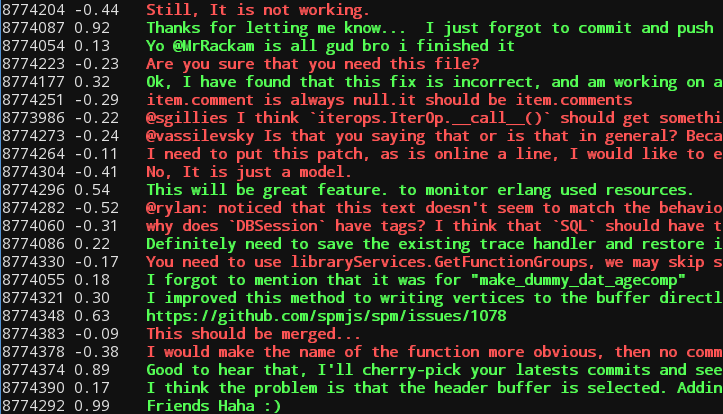
\includegraphics[width=0.5\textwidth]{Images/Classifier.png}
  \caption{Visual output of the classifier tool. Each line of the output
           consists of the ID, the sentiment score and the textual content of
           a commit comment. A negative score yields red text in the output,
           whereas a positive score yields green text in the
           output.}\label{fig:classifier-output}
\end{figure}

Another use of the tool is to cross-validate the chosen classifier. For a given 
number of folds, the labeled dataset is split into that number of folds, and 
the same number of models are created. Each model is trained with one fold and 
then the scores on the rest of the folds are predicted. We then compare these 
predictions with the actual labels of each comment, and calculate the average 
correctness of the models.

The predictions themselves can again be analyzed using the reducer and plotter, 
similar to the naive analyzer output. The classifier can therefore be run using 
MapReduce as well. When using the preprocessor with MPI to retrieve all commit 
comments dumps in a distributed way, one can also run the classifier to predict
the comments in the dumps on the worker nodes.

\subsection{MapReduce and reducer}\label{sec:reducer}
MapReduce~\cite{dean2004mapreduce} is a component of Hadoop which allows to
create two kinds of jobs: mappers and reducers. The mappers receive input on
which they perform calculations and their output is sorted and split up to the
reducer jobs, which can, for example, make counts or perform other aggregation
tasks. This allows for distributed computation in phases.

We make use of MapReduce for our prediction and analysis tools. The naive 
analyzer from Section~\ref{sec:analyzer} and the classifier described in 
Section~\ref{sec:classifier} conform to the input and output requirements of 
a mapper. The output can be keyed by a certain group and the sorting can take 
into account which part is the key and which part is a value.

The combiner part of MapReduce performs the sorting, so that the output becomes 
suitable for the reducer. This script simply counts the frequency of a certain 
score in the file, and the output is then also sorted on those scores. In case 
of groups, the input is sorted on each group value first, thus the frequency
counts also happen per group and per score. This makes it possible to plot the
counts in a frequency plot or to visualize the relative scores of each group.

\subsection{Plotter}\label{sec:plotter}
In order to visualize the predictions and other outputs of the various 
components, we implement a plotting framework that is able to create multiple 
types of plots in PDF format. The framework is based on the \textsc{matplotlib} 
library~\cite{hunter2007matplotlib}. There are three ``groups'' of plots, the 
first one being the \texttt{score} group which generates a frequency plot. The 
input of this group is a tab-delimited file with predictions, which we generate 
using the analyzer or classifier and the reducer from 
Section~\ref{sec:reducer}. The plot output is a bar chart of the frequencies of 
each score bin, and this discrete histogram is augmented with a smooth curve.

Another group that the plotter recognizes is the same group given to the 
analyzer or classifier, specifically the \texttt{language} group. This allows 
us to obtain a stacked bar chart which displays the positive and negative 
ratios of the relative scores in each language. This plot type is used in the 
experiment in Section~\ref{sec:sentiment-analysis-per-language}.

The final plot type is the \texttt{algo} group, which generates multiple plots 
for each experiment that the experiment runner in 
Section~\ref{sec:experiment-runner} runs. For each experiment in the resulting 
JSON file of the experiment runner with various combinations of parameters, we 
create a plot with the average scores and standard deviations calculated from 
the cross-validation runs of each parameter combination. We use these plots in 
our experiments that compare the classifiers in 
Section~\ref{sec:most-accurate-classifier}.

\subsection{Experiment runner}\label{sec:experiment-runner}
Determining the best classifier to use from the \textsc{scikit-learn} toolkit is
essential for obtaining reliable classifications. Since our labeled training
set containing 2000 labeled commit comments is relatively small, it is possible
to explore a large number of different classifiers with many different
combinations of parameters. We therefore develop an experiment runner that
performs cross-validation (five folds by default, but the number of folds is
configurable) on all classifiers and parameter combinations listed in a
manifest file.

The experiment runner, as mentioned before, depends on the availability of
a manifest file, which is a JSON file that contains an array of objects
describing the classifier and the parameters to test. An example entry
of the manifest file is the following:

\begin{verbatim}
{
  "class_name": "AdaBoostClassifier",
  "module": "sklearn.ensemble.weight_boosting",
  "name": "Ada Boost classifier",
  "parameters": {
    "n_estimators": [
      10,
      50,
      100,
      250,
      500
    ],
    "learning_rate": [
      0.1,
      0.2,
      0.3,
      0.4,
      0.5
    ]
  }
}
\end{verbatim}

In a manifest entry we mention the class name of the classifier to test, the
module to which the classifier belongs, the human-readable name of the 
classifier and the parameters of the classifier that that experiment runner can 
test. In the example above, we have two parameters, namely {\tt n\_estimators} 
and {\tt learning\_rate}. The manifest entry essentially indicates that we 
perform cross-validation for the Ada Boost classifier with all possible 
combinations of the parameter values. In this case we perform 25~runs, namely 
one with {\tt n\_estimators = 10} and {\tt learning\_rate = 0.1}, one with
{\tt n\_estimators = 10} and {\tt learning\_rate = 0.2}, and so on.

We use a manifest file that contains 15 different classifiers. The
parameters and the values of the parameters to test have been determined by
studying the \textsc{scikit-learn} toolkit documentation. The experiment runner
reads the manifest file and performs cross-validation for each mentioned
classifier and for each parameter combination. The results of the
cross-validation are written to an output JSON file that the plotter from
Section~\ref{sec:plotter} can take as input and, using the `algo' group,
creates an SVG plot for each classifier.

Using the experiment runner on the training set gives an indication of
how accurate each classifier is on our dataset. The classifier and
parameter combination that yields the highest accuracy is used for the
final classifier.

\subsection{Labeler}\label{sec:labeler}
As a labeled training set does not yet exist for the GitHub commit comments
dataset, we have to make one ourselves. In order to streamline this process
and to collaborate on the effort, we implement a labeler. We use the commit
comments dump from 29--01--2015 to create our labeled training set.

The labeler loads this dataset, presents each commit comment individually to
the user, displays a prediction based on the naive word list approach and asks
the user whether or not he or she agrees with the prediction. If so, simply
pressing Enter stores the label for that commit comment. If not, the user
can enter `p' for positive, `n' for negative, `t' for neutral and `u' for
unknown, thereby overriding the prediction. We mark commit comments as unknown
such that the classifier ignores them if they do not contain useful content,
for instance comments containing only names of variables. We do not want to
confuse the classifier with those comments during the training phase to avoid
mispredictions.

In order to collaborate on the effort, the commit comments along with their
labels are stored in JSON format. The labeler automatically resumes where
the last collaborator left off. For example, if the first collaborated labeled
up until commit comment 500, then a second collaborator would resume labeling
at commit commit 501, thereby skipping already labeled commit comments. The
JSON file with the commit comment labels can therefore easily be put in a
version control system such that any user can use the labeler and continue 
where others left off.

\subsection{MPI}\label{sec:mpi}
Message Passing Interface (MPI) is a protocol for creating communication 
channels between instances of a parallelized program. These channels can be 
created in various ways, depending on the platform and the instantiation of the 
program. One can use shared memory when the instances are threads. In the case 
that we instantiate separate processes, an inter-process communication channel 
allows for data sharing. Finally, if the processes are on different worker 
nodes, a network protocol such as SSH resolves the communication. Agent 
forwarding and key-based authentication ensure that none of the connections 
require interactive password prompts.

OpenMPI~\cite{gabriel2004openmpi} is one implementation of MPI which supports 
all these communication channels. It executes multiple instances of another
program in parallel. In case the specific program uses the available MPI
bindings, then the communication channels allow data sharing and program
synchronization. We use the \textsc{mpi4py} library for
Python~\cite{dalcin2008mpi4py} in order to use the MPI bindings within our 
programs.

We specifically use MPI and the data communication in the preprocessor from 
Section~\ref{sec:preprocessor}. We dispatch jobs for each dump that we want to 
download, extract and process. When a worker node has finished a job, it sends 
a message to the master process, which awakens from an idle polling loop. The 
master process then either sends a new job to the worker node based on the dump 
date, or signals the worker that it is done if all jobs have been assigned. The 
list of dumps is sorted on their compressed file size, so that the worker nodes 
first process the largest tasks. When a worker node finishes a job earlier than 
others, then it receives a new job before a worker node that is processing a
larger dump. This yields an automatic load-balancing based on the processing
time of each dump.

The classifier from Section~\ref{sec:classifier} also supports running with 
MPI\@. In this case, all communications happens using standard output streams
and shared files. The classifier can detect commit comments dumps that the 
MPI-enabled preprocessor extracts on worker nodes on their local hard drives, 
and predict the messages in each of them individually, based on a trained 
model. The predictions are then collected and can then be used in other 
components.

\section{Experiments and results}\label{sec:experiments-and-results}
% TODO: Explain experiments: timing, memory?, analyzer/classifier frequency 
% plots (in case we need more experiments...)?
In this section, we introduce the experiments that we perform with the 
framework from Section~\ref{sec:implementation} upon the GitHub commit comments 
dataset described in Section~\ref{sec:dataset}. We measure and compare the 
running time and memory usage of our components on different platforms and 
distributed computing techniques in Section~\ref{sec:time-and-memory-usage}. 
After thoroughly testing our framework, we use it to determine the most 
accurate classifier upon the dataset in 
Section~\ref{sec:most-accurate-classifier}. Finally, we use the observations 
made in these experiments and apply the components of our framework to the 
problem of finding the most positive and most negative languages based on the 
main programming language of each repository on GitHub. The results and 
observations from this experiment are shown in 
Section~\ref{sec:sentiment-analysis-per-language}.

\subsection{Measuring time and memory usage of the framework}\label{sec:time-and-memory-usage}
\ldots

% Some notes: for MPI, the commit comments preprocess runs use 17 dumps instead 
% of just 1 as we do on the other platforms. Furthermore, the MPI run of the 
% classifier and reducer components use the sum of all the worker nodes, 
% including the master and the MPI managing process. The MapReduce timing is 
% also based on the Hadoop job and resource monitoring system as well as the 
% resource information of individual job tasks provided by Hadoop's statistics.
% Need to explain the difference between real and user/sys clearly, with 
% examples etc.
\begin{table}[h!]
  \centering
  \begin{tabular}{l l l l l}
    \toprule
    \textbf{Component} & \textbf{Baseline} & \textbf{MapReduce} &
    \textbf{Baseline languages} & \textbf{MPI languages $\times$ 17} \\
    \midrule
    Preprocessor           & 2 minutes & ---    & 22 hours    & 7 hours    \\
    \quad Repositories     & ---       & ---    & 20h 58m 15s & 6h 56m 18s \\
    \quad Commit comments  & 1m 52s    & ---    & 1h 9m 50s   & 1h 6m 29s  \\
    Analyzer               & 1m 3s     & 1m 8s  & ---         & ---        \\
    Classify, sort, reduce & 1m 6s     & 1m 46s & 1m 9s       & 1m 49s     \\
    \quad Classifier       & 1m 2s     & ---    & 1m 2s       & 1m 18s     \\
    \quad Reducer          & 0.2s      & ---    & 0.2s        & 2s         \\
    \bottomrule
  \end{tabular}
  \caption{Real time of components using various distributed platforms.}
  \label{tab:component-real-time}
\end{table}
\begin{table}[h!]
  \centering
  \begin{tabular}{l l l l l}
    \toprule
    \textbf{Component} & \textbf{Baseline} & \textbf{MapReduce} &
    \textbf{Baseline languages} & \textbf{MPI languages $\times$ 17} \\
    \midrule
    Preprocessor           & 1 minute  & ---    & 8.5 hours   & 17 hours   \\
    \quad Repositories     & ---       & ---    & 8h 26m 1s   & 9h 40m 30s \\
    \quad Commit comments  & 1m 10s    & ---    & 15m 57s     & 7h 32m 49s \\
    Analyzer               & 1m 3s     & 1m 23s & ---         & ---        \\
    Classify, sort, reduce & 1m 4s     & 1m 46s & 1m 5s       & 10m 23s    \\
    \quad Classifier       & 1m 3s     & 1m 40s & 1m 3s       & 10m 9s     \\
    \quad Reducer          & 0.2s      & 10s    & 0.2s        & 2s         \\
    \bottomrule
  \end{tabular}
  \caption{Summed user and system time of components using various distributed 
  platforms.}
  \label{tab:component-user-sys-time}
\end{table}
\begin{table}[h!]
  \centering
  \begin{tabular}{l r r r r}
    \toprule
    \textbf{Component} & \textbf{Baseline} & \textbf{MapReduce} &
    \textbf{Baseline languages} & \textbf{MPI languages $\times$ 17} \\
    \midrule
    Preprocessor           & 16 MB   & ---    & 543 MB & 2.2 GB  \\
    \quad Repositories     & ---     & ---    & 356 MB & 1681 MB \\
    \quad Commit comments  & 16.4 MB & ---    & 187 MB & 563 MB  \\
    Analyzer               & 7.5 MB  & 956 MB & ---    & ---     \\
    Classify, sort, reduce & 212 MB  & 942 MB & 222 MB & 1.7 GB  \\
    \quad Classifier       & 199 MB  & ---    & 208 MB & 1673 MB \\
    \quad Reducer          & 4.0 MB  & ---    & 4.0 MB & 4.0 MB  \\
    \bottomrule
  \end{tabular}
  \caption{Memory usage of components using various distributed platforms.}
  \label{tab:component-mem}
\end{table}
% Note, when we wish to display the output of the classifier with the id group, 
% the test data has to be converted to a list in order to show the prediction 
% along with the original message. This increases the memory to 282 MB for the 
% classifier only, an increase of 83 MB. The classifier component's memory 
% usage is also very dependent on the actual classifier model used. MapReduce 
% has a lot of overhead from the Java stack it is on, and provides little 
% detail on memory usage.

\subsection{Determining the most accurate 
classifier}\label{sec:most-accurate-classifier}
Before we are able to classify commit comments, it is important to determine
the most accurate classifier to use on our dataset. In order to consider as
many combinations of classifier and parameters as possible, we have implemented
an experiment runner as described in Section~\ref{sec:experiment-runner}.

The experiment runner performs five-fold cross-validation using the 
2000~entries in the labeled training set for each combination of classifier and 
parameters. Since we have discrete classes in our labeled dataset (positive, 
negative or neutral), we use classifiers instead of regressors. A regressor 
gives relative scores instead of discrete classes, and this would artificially 
worsen the scores on the cross-validation test folds. We assume that the 
regressor variants of the available classifiers from \textsc{scikit-learn} 
behave similarly to the classifiers, of which we make use in the subsequent 
experiment in Section~\ref{sec:sentiment-analysis-per-language}.

We execute the experiment runner, which takes several minutes to about an hour 
to complete all its tasks. For each combination of classifier and 
a predetermined set of values for the available parameters, we calculate the 
average accuracy and the standard deviation of the five cross-validation runs. 
We store these results in a JSON file. The plotting framework from 
Section~\ref{sec:plotter} is able to read this JSON file and create separate 
plots for each classifier, and in case there are many combinations of 
parameters, for each value of a certain parameter. This allows us to visually 
inspect the results and to compare the effect of different parameters in 
combination with the same algorithm. Figure~\ref{fig:classifiers} shows the 
three most accurate classifiers on the labeled training set.

\begin{figure}[h!]
  \centering
  \begin{subfigure}{.48\textwidth}
    \centering
    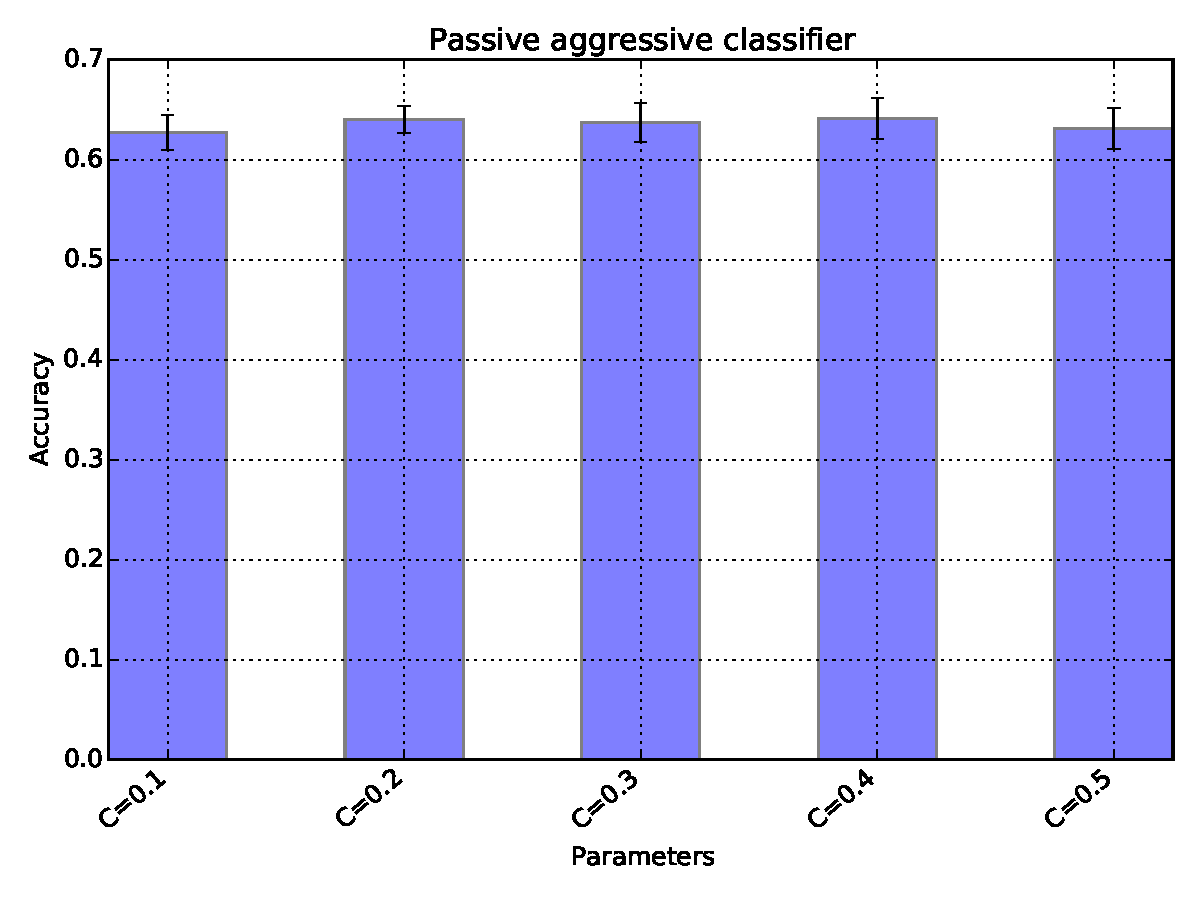
\includegraphics[width=\textwidth]{Images/Passive_aggressive.pdf}
    \caption{Passive aggressive classifier}\label{fig:classifiers-passive-aggressive}
  \end{subfigure}
  \begin{subfigure}{.48\textwidth}
    \centering
    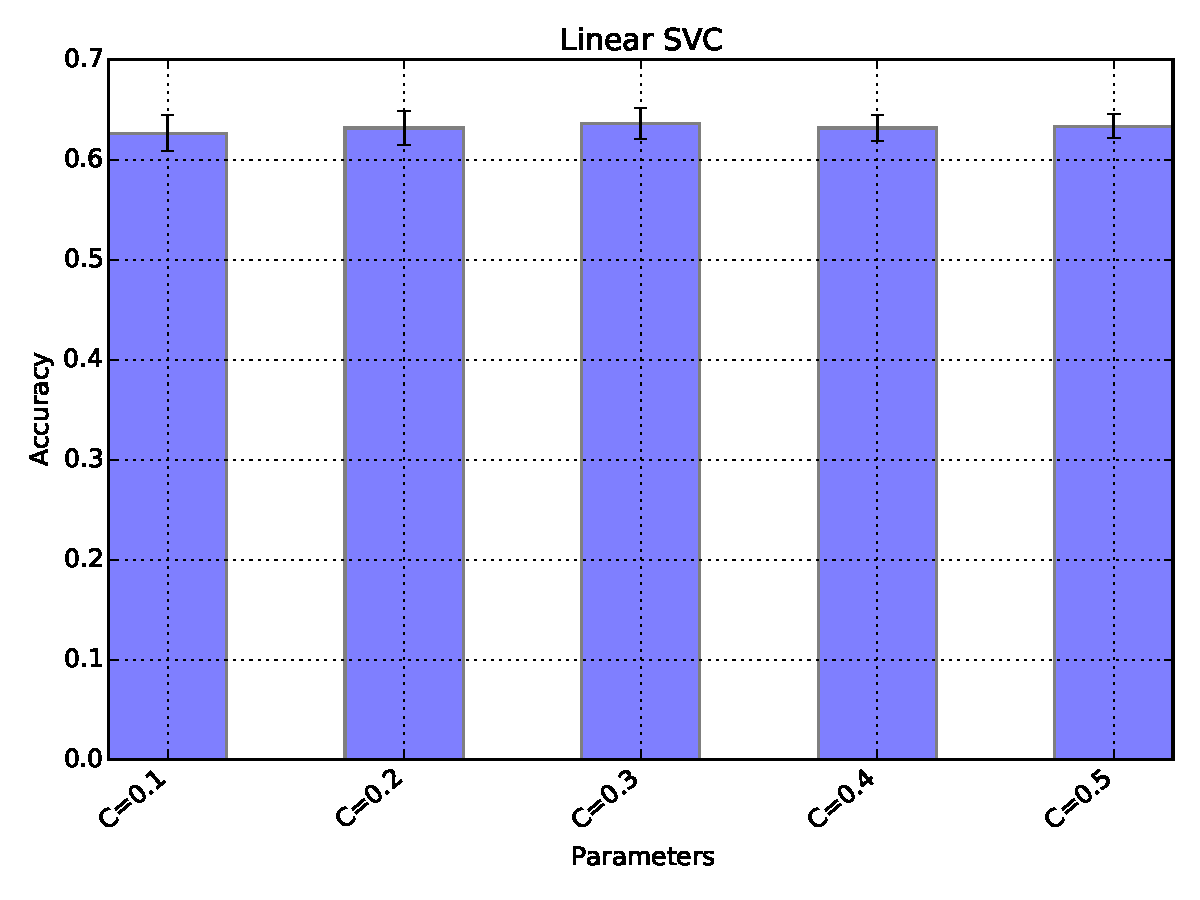
\includegraphics[width=\textwidth]{Images/Linear_SVC.pdf}
    \caption{Linear SVC}\label{fig:classifiers-linear-svc}
  \end{subfigure} \\
  \vspace{0.5cm}
  \begin{subfigure}{.48\textwidth}
    \centering
    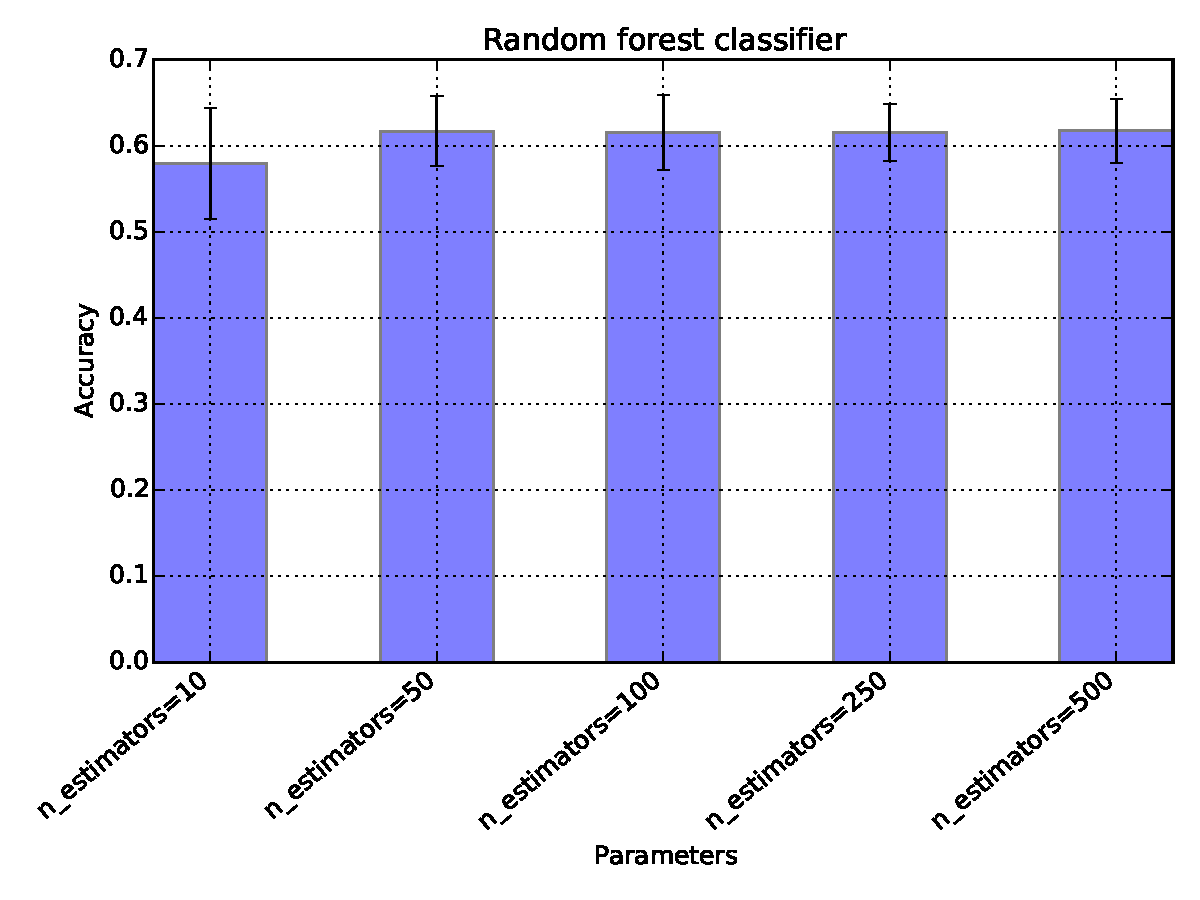
\includegraphics[width=\textwidth]{Images/Random_forest.pdf}
    \caption{Random forest classifier}\label{fig:classifiers-random-forest}
  \end{subfigure}
  \caption{Three most accurate classifiers on the labeled training set, based
           on five-fold cross-validation. Accuracy values range 
           between~0~and~1, indicating 0\%~and~100\%~accuracy, 
           respectively.}\label{fig:classifiers}
\end{figure}

We observe from the plots that these three classifiers yield very similar
accuracies on the labeled training set, with an average of 63\%~accuracy.
The plots also show that all three classifiers are relatively stable,
meaning that changing parameters has a very low impact on the accuracy
and standard deviation. We see that the passive aggressive classifier and
linear SVC are almost identical, whereas the accuracy of the random forest
classifier is slightly lower and the standard deviation is slightly higher,
especially when the number of estimator trees is small.

The random forest classifier fits several decision tree classifiers on
samples of the dataset. Averaging is applied to improve the accuracy and
to prevent overfitting~\cite{breiman2001randomforests}. We find however that 
the individual decision trees often become very large on our dataset, with 
a long tail where a node keeps on being split on a condition in order to 
improve the accuracy within that node. After tuning parameters, the trees have 
fewer nodes, but there are still nodes that have too many splits in their 
subtree.

Linear SVC is a support vector machine, which is especially well-suited for 
scaling up to a large number of samples. The passive aggressive classifier 
works by keeping a model if the prediction is correct and by updating the model 
when a sample is misclassified~\cite{crammer2006passive}. After careful 
comparison of the classifiers, we decide to use the passive aggressive 
algorithm with regularization parameter $C = 0.4$ for the classifier component 
as it is slightly more accurate than the linear SVC.

\subsection{Performing sentiment analysis per language}\label{sec:sentiment-analysis-per-language}
For this experiment, we apply our distributed sentiment analysis framework to
analyze the ratio of positive and negative commit comments per programming
language. Performing such an analysis might be useful for gaining insight into 
the satisfaction of the developers and determining problems with programming 
languages. For instance, if many reviewers are negative about a certain 
language, inspection of the commit comments could indicate reasons for this, 
which can be addressed by the designers of the programming language, such as 
addressing shortcomings that make implementation of algorithms or bugfixing
more difficult. Python and PHP are examples of mature programming languages
that are constantly updated based on new specifications and wishes from the
community.

We combine the commit comments dataset and the repositories dataset described 
in Section~\ref{sec:dataset}. Each commit comment is augmented with the main 
programming language of the repository that the commit belongs to. This 
experiment also shows the potential of our distributed approach. The large
amount and variety of data requires us to use almost all available tools in the
framework shown in Section~\ref{sec:implementation}. Not only do we need to
preprocess the commit comments dataset, but first we must preprocess the
repositories dataset such that we have the main language of each repository
available when we preprocess the commit comments data. Our framework supports
processing both types of dumps in a distributed manner.

We utilize eight nodes of DAS-3 for this experiment, including the fileserver 
node which acts as a master node. We start by preprocessing the repositories 
dataset on the worker nodes as outlined in Section~\ref{sec:mpi}. This task 
processes 17~dumps containing the repositories and creates a shelve for each of 
them. The shelves only store the main language of each repository. After 
completion of the task, we preprocess the commit comments dataset on the worker 
nodes too. First, we merge the shelves into one shelve, so that we can easily 
look up the language of each repository. We add the language to each commit 
comment in the process, by inspection of the repository it is from, based on 
the {\tt url} attribute. Once this task is also completed, we obtain a JSON 
file for every dump that contains for each commit comment the text and the main 
language of the repository it belongs to.

These files are kept on the worker nodes on which the preprocessor extracted 
them. We use the classifier component with MPI as well, in order to pass each 
file to the classifier component by running an instance of the classifier with 
the {\tt language} group on each node. We use a model of the passive aggressive 
regressor from \textsc{scikit-learn} that we train beforehand. We show in 
Section~\ref{sec:most-accurate-classifier} that the classifier version of the 
passive aggressive algorithm appears to have the best fit for our dataset. We 
use the regressor variant since this gives us relative scores for each commit 
comment, which improves the results of our comparisons of the languages. The
output of the classifier consists of single lines with on each line the main
language name and the score of one commit comment. The plotting framework
takes this output as input and generates the plots in 
Figure~\ref{fig:language-pos} and Figure~\ref{fig:language-neg}, which show
the 20~most positive and most negative languages based on the comment
comments, respectively.

\begin{figure}[h!]
  \centering
  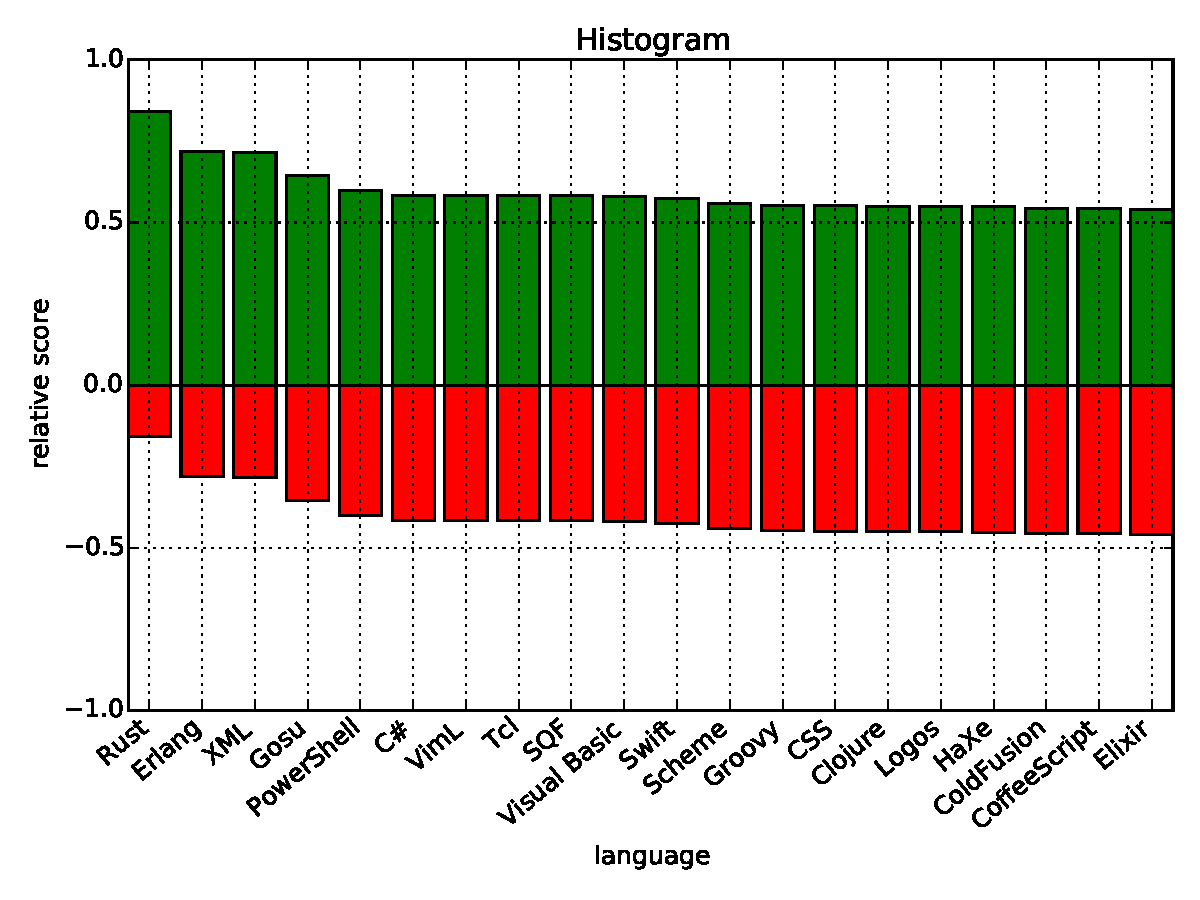
\includegraphics[width=0.8\textwidth]{Images/Positive_languages_passive_aggressive.pdf}
  \caption{Top 20 of programming languages with the most positive commit comments.}\label{fig:language-pos}
\end{figure}

\begin{figure}[h!]
  \centering
  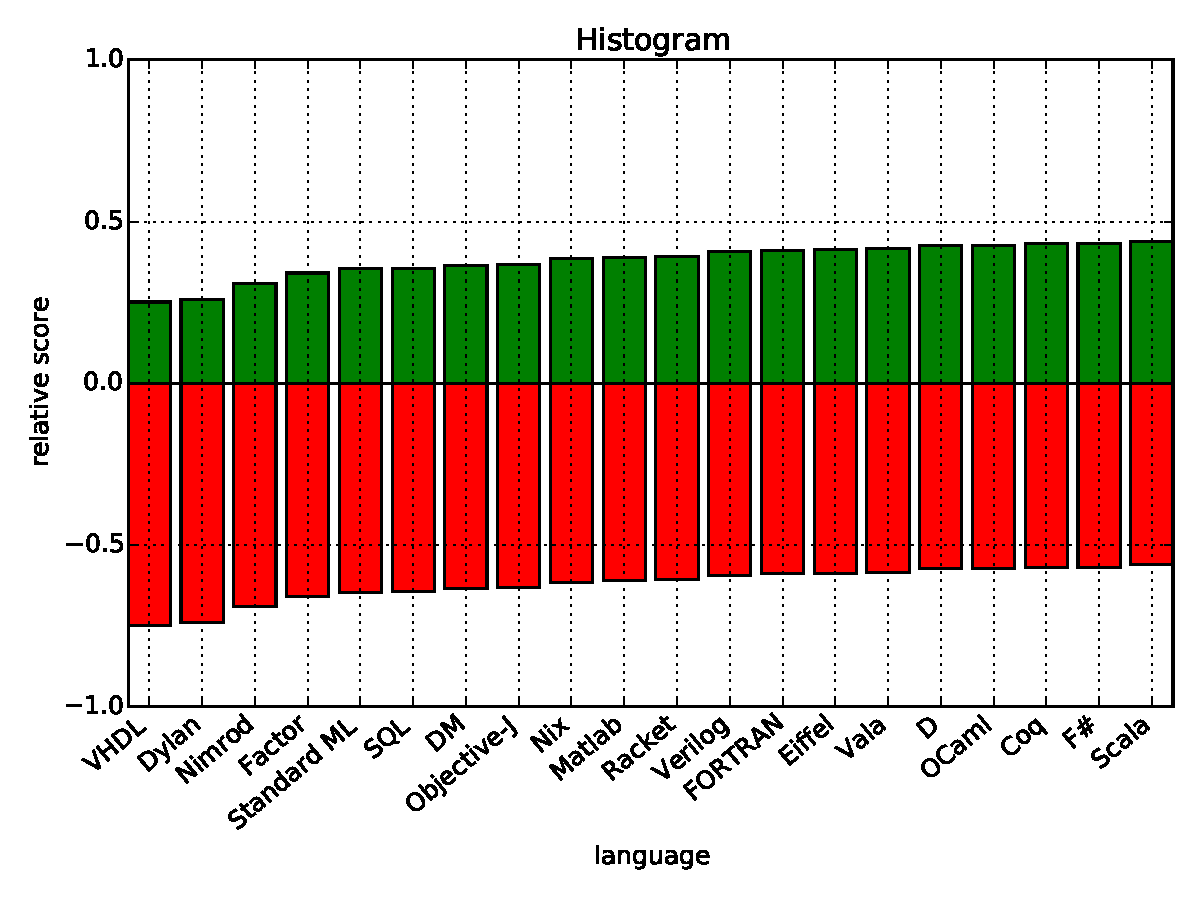
\includegraphics[width=0.8\textwidth]{Images/Negative_languages_passive_aggressive.pdf}
  \caption{Top 20 of programming languages with the most negative commit 
  comments.}\label{fig:language-neg}
\end{figure}

The two most positive languages are Rust and Erlang, which are interesting 
appearances among the top~20. First, Rust is a fairly new language which is 
under development on GitHub. We noticed by manual inspection
of the commit comments that many commit comments consist of output from testing 
bots. However, it can be seen as positive if all tests pass and as negative if 
all tests fail, and clearly the tests often pass for those languages, which is 
indeed a positive sign. The same also applies to the Erlang language, where we 
also find that many comments are simply very positive and even excited about 
the implementation of new features that are possible using the language. The 
top~20 of the most positive languages also contains other new languages for 
which this ease of use also applies.

Among the most negative languages we have VHDL and Matlab as interesting 
appearances. Developers often seem to be annoyed by problems when changing
code in these languages, and are often surprised about the way certain bugs 
are resolved in the code.

We see many small and relatively unknown languages in both plots. This can be
improved by changing our weighting scheme to take the group size more into
account. Currently we do filter languages that have very few comments, but
adding more restrictions on the number of comments per language makes smaller
languages like Dylan and Nimrod unlikely to appear in the plots. Clearly,
more weighting schemes are possible and our plotting framework allows for
these modifications, but we have chosen this weighting scheme for simplicity
and to be able to list smaller languages too.

\section{Conclusion}\label{sec:conclusion}
We have implemented a framework in Python for distributed sentiment analysis on
the GitHub commit comments dataset. Our framework includes two different
approaches for performing sentiment analysis, namely a naive positive and
negative word list approach and a classifier approach. We have discussed the
components available in the framework, such as the preprocessor, the naive
analyzer, the classifier and the experiment runner.

For the classifier approach we have evaluated 15~different classifiers,
including many combinations of parameters, with five-fold cross-validation on
a manually labeled training set of 2000~commit comments. These experiments show
that the passive aggressive classifier with $C = 0.4$ is the most accurate on 
the commit comments dataset, while other classifiers such as the random forest 
classifier also yield high accuracies.

We have performed another experiment to show the potential of our framework by
performing sentiment analysis on all available commit comments and then grouping
labels by the main programming language of the repository that each commit
belongs to. We have generated plots of the 20~languages where the overall
developer sentiment is most positive and where it is most negative.

\subsection{Future research}\label{sec:future-research}
There are several possible extensions that we leave for future research. The
first extension is the application of principal component analysis (PCA) and
working with sentiments in more dimensions. This means that we are not labeling
commit comments as strictly positive, negative or neutral, but instead we use
emotion categories such as `happy', `disappointed' or `angry'. This approach
makes the results of the sentiment analysis more specific, and algorithms that 
specifically deal with these multiple classes might increase the overall 
accuracy.

The second possible extension is to apply the framework to specific users,
repositories, communities or discussions. This scope limitation makes it
more feasible to, for example, implement a system that performs sentiment
analysis on a data stream in realtime. This gives some practical use cases such 
as determining the atmosphere of a discussion, which can be a guideline as to 
whether a suggested code change seems to be accepted by the community or not.

Finally, further research could go into a comparison with other classifiers,
such as neural networks and natural language processing, including word 
stemming. We can also research other interpretations of the used classifiers, 
such as the out-of-bag error for the random forest classifier.

\section*{References}\label{sec:references}
\printbibliography[heading=none]

\newpage

\appendix
\section{Appendix}\label{app:appendix}
This appendix is based on an instruction file that accompanies the 
code of our implementation from Section~\ref{sec:implementation}. The code can 
be retrieved from a Git repository at 
\url{https://github.com/timvandermeij/sentiment-analysis}. This repository 
contains all code necessary to perform sentiment analysis on a large dataset of 
Git commit comments from GitHub (\url{http://www.ghtorrent.org}). The code is 
meant to be run on the Distributed ASCI Supercomputer 3 (DAS-3) at LIACS, and 
makes use of Apache Hadoop's HDFS and MapReduce to perform the sentiment 
analysis, but has also been tested to work on other hardware and software 
platforms.

\subsection{Prerequisites}\label{app:prerequisities}
The version numbers mentioned below have been verified to work. Different
versions might also work.

\begin{itemize}
  \item Git 1.7.1 or 2.3.x
  \item Python 2.7.9 with libraries (see installation notes in 
    Section~\ref{app:python} for details)
\end{itemize}

\subsection{Cloning the repository}\label{app:cloning-the-repository}
The first step is to clone the repository to obtain a local copy of the code. 
Open a terminal window and run the following commands.

\begin{verbatim}
$ git clone https://github.com/timvandermeij/sentiment-analysis.git
$ cd sentiment-analysis
\end{verbatim}

\subsection{Running the code}\label{app:running-the-code}
All code is written in Python. To run the simple sentiment analysis program, execute:

\begin{verbatim}
$ python preprocess.py
$ echo '{"body":"Yay, it is working perfectly!"}' | python analyze.py score
\end{verbatim}

For the default group of \texttt{id} and the group \texttt{score}, running
\texttt{preprocess.py} only needs to be done once. If all required data is
available, \texttt{preprocess.py} will do nothing.

The output of the analysis program are lines containing scores between $-1$ and 
$1$, where $-1$ indicates that the message is negative, $1$ indicates that the 
message is positive and $0$ indicates that the message is neutral. The output 
can also contain grouping data or some visualization of the message.

Instead of using a single line as input, one can give a file to read as standard
input as follows:

\begin{verbatim}
$ python analyze.py < commit_comments-dump.2015-01-29.json
$ python classify.py score < commit_comments-dump.2015-01-29.json
\end{verbatim}

The latter \texttt{classify.py} script uses a classifier to predict the scores 
using a labeled dataset. Both programs work in a similar manner. This script 
requires the 2015--01--29 commit comments dump in order to 
cross-reference the labels with the messages. The classification itself can be 
run on any dump, and the script will filter any already labeled messages before 
prediction.

The output can be given to the \texttt{reducer.py} script, but only if it has 
been sorted on the first column of the output (the group or the score of the 
line). This can be done using MapReduce as described later on, or by passing 
the output through \texttt{sort}. The \texttt{reducer.py} script generates 
a histogram of frequencies of the scores which can be passed to 
\texttt{plot.py} to make a graph of the frequencies.

\subsubsection{Groups}\label{app:groups}
The code by default uses the \texttt{id} of a record as its group. This means 
that only the analyzer and classifier will do something useful. The reducer and 
plot scripts do not work nicely when the data is grouped this way. In order to 
group the classified targets with something else, pass another group, such as 
\texttt{score} or \texttt{language}, to all relevant scripts.

Note that for the \texttt{language} group, the preprocessor needs to retrieve 
more data, which can be done with \texttt{python preprocess.py repos language} 
and then again use \texttt{python preprocess.py commit\_comments language}. 
These commands can also be distributed using MPI, in order to retrieve and 
process multiple dump files in parallel processes. Note that it is only 
necessary to parallelize the second command if one wants to receive all the 
commit comments dumps, whereas working with the 2015--01--29 dataset is 
usually enough. The MPI parallelization can be done on one machine using 
\texttt{mpirun -n <num\_processes> python preprocess.py 
repos language}. The instructions for running the preprocessor on distributed 
worker nodes are given in Section~\ref{app:mpi}, where the command is 
\texttt{pympi <num\_processes> preprocess.py "repos 
language" -{}-hostfile hosts -{}-map-by node}.

\subsubsection{Running the code in MapReduce}\label{app:mapreduce}
This section assumes that the installation notes in 
Section~\ref{app:installation-notes} have already been followed and all 
dependencies and scripts are set up. The exact commands to call the MapReduce 
scripts, for various group parameters, are given in this section.

First of all, ensure that the data sets are on the HDFS:

\begin{verbatim}
$ hdfs dfs -put commit_comments-dump.2015-01-29.json
$ hdfs dfs -put commit_comments-dump.2015-01-29.labeled.json
$ hdfs dfs -put words/positive.txt words/positive.txt
$ hdfs dfs -put words/negative.txt words/negative.txt
\end{verbatim}

Now, one can start a MapReduce job which classifies each record in the dataset 
and then counts the frequency of each score as follows:

\begin{verbatim}
$ pyhadoop commit_comments-dump.2015-01-29.json score classify.py reducer.py \
  score score -file commit_comments-dump.2015-01-29.labeled.json -file \
  commit_comments-dump.2015-01-29.json -file utils.py -file algorithms.json
\end{verbatim}

For the naive analyzer, use \texttt{analyze.py} instead of 
\texttt{classify.py}, and add the following arguments to the 
command:
\begin{verbatim}
-file \"\$HDFS\_URL/words/positive.txt\#words/positive.txt\" \
-file \"\$HDFS\_URL/words/negative.txt\#words/negative.txt\"
\end{verbatim}

In order to count frequencies of scores within a specific group, use the 
following command:

\begin{verbatim}
$ pyhadoop commit_comments-dump.2015-01-29.json score_lang classify.py \
  reducer.py language language -D stream.num.map.output.key.fields=2 \
  -file commit_comments-dump.2015-01-29.labeled.json -file \
  commit_comments-dump.2015-01-29.json -file utils.py -file algorithms.json
\end{verbatim}

This ensures that MapReduce knows which parts of the outputs are keys and which 
are values.

\subsection{Installation notes for the DAS-3}\label{app:installation-notes}
This section describes how to set up all dependencies for running the Python
code on the Distributed ASCI Supercomputer 3 at LIACS\@. Among others, this
gives instructions for installing Python 2.7 that can be run in a virtual
environment, Hadoop configuration and MPI.

\subsubsection{Python}\label{app:python}
Compile Python (version 2.7.9) from source:

\begin{verbatim}
$ wget https://www.python.org/ftp/python/2.7.9/Python-2.7.9.tgz
$ tar xzvf Python-2.7.9.tgz
$ cd Python-2.7.9
$ ./configure --prefix=$HOME/.local
$ make
$ make install
$ rm Python-2.7.9.tgz
\end{verbatim}

\subsubsection{Virtualenv}\label{app:virtualenv}

Install \textsc{virtualenv} using \textsc{pip} and create a virtual environment 
called \texttt{python} that we can distribute over the nodes using HDFS:

\begin{verbatim}
$ pip install --user virtualenv
$ mkdir /scratch/scratch/{username}
$ cd /scratch/scratch
$ chmod 700 {username}
$ cd {username}
$ ~/.local/bin/virtualenv -p ~/.local/bin/python2.7 python
$ ~/.local/bin/virtualenv --relocatable python
\end{verbatim}

\subsubsection{OpenMPI}\label{app:openmpi}
Compile OpenMPI from source:

\begin{verbatim}
$ cd ~
$ wget http://www.open-mpi.org/software/ompi/v1.8/downloads/openmpi-1.8.4.tar.gz
$ tar xzvf openmpi-1.8.4.tar.gz
$ cd openmpi-1.8.4/
$ ./configure --prefix=$HOME/.local
$ make
$ make install
$ rm openmpi-1.8.4.tar.gz
\end{verbatim}

\subsubsection{OpenBLAS}\label{app:openblas}
Compile OpenBLAS from source:

\begin{verbatim}
$ cd ~
$ git clone git://github.com/xianyi/OpenBLAS
$ cd OpenBLAS && make FC=gfortran
$ make PREFIX=$HOME/.local install
\end{verbatim}

\subsubsection{Update Bash configuration}\label{app:update-bashrc}
Append the following segment to \texttt{$\sim$/.bashrc}:

\begin{verbatim}
if [ "$HOSTNAME" = "fs.das3" ]; then
    export SCRATCH="/scratch/scratch/{username}"
else
    export SCRATCH="/scratch/{username}"
fi
alias activate="source $SCRATCH/python/bin/activate"
export PATH="$PATH:$HOME/.local/bin:/mounts/CentOS/6.6/root/usr/bin"
export PATH="$PATH:$SCRATCH/python/bin:$SCRATCH/opt/bin:$SCRATCH/opt/lib"
export LIBRARY_PATH="$HOME/.local/lib:$SCRATCH/opt/lib"
export LD_LIBRARY_PATH="$HOME/.local/lib:$SCRATCH/opt/lib"
export CPATH="$HOME/.local/include:$SCRATCH/opt/include"
export PKG_CONFIG_PATH="$HOME/.local/lib/pkgconfig:$SCRATCH/opt/lib/pkgconfig"
export BLAS="$SCRATCH/opt/lib/libopenblas.a"
\end{verbatim}

Then use \texttt{source $\sim$/.bashrc} to reload the configuration.

\subsubsection{Python libraries}\label{app:python-libraries}
Activate the virtual environment:

\begin{verbatim}
$ activate
\end{verbatim}

We now have a Python 2.7 virtual environment running, but \textsc{pip} is still 
from Python 2.6. In order to fix this, run the following:

\begin{verbatim}
(python)$ cd $SCRATCH
(python)$ wget https://bootstrap.pypa.io/get-pip.py
(python)$ python get-pip.py -U -I
\end{verbatim}

This installs \textsc{pip} for Python 2.7, which is less likely to give 
troubles when we are installing or upgrading dependencies. Now first install the following dependencies:

\begin{verbatim}
(python)$ pip install cython
(python)$ pip install readline
(python)$ pip install pymongo
\end{verbatim}

Next we need to compile \textsc{NumPy} from source as we need it to work with 
OpenBLAS\@. This BLAS implementation not only performs better than standard
BLAS installations according to benchmarks at 
\url{http://stackoverflow.com/a/7645939}, but \textsc{SciPy} requires it 
since Lapack/BLAS are not installed on the DAS-3. Follow the instructions 
from step~2 onward from \url{http://stackoverflow.com/a/14391693}. Make sure to 
use \texttt{/home/\string{username\string}/.local} for the paths.

If that is done (make sure to test that it is working) we continue installing 
the remaining dependencies. Make sure to use \texttt{--no-deps} for libraries 
that depend on \textsc{NumPy}, since these often attempt to overwrite our 
source installation of \textsc{NumPy}.

\begin{verbatim}
(python)$ pip install --no-deps scipy
(python)$ pip install --no-deps pandas
(python)$ pip install python-dateutil
(python)$ pip install pytz
(python)$ pip install --no-deps scikit-learn==0.16b1
(python)$ pip install --no-deps numexpr
(python)$ pip install --no-deps matplotlib
(python)$ pip install pyparsing
(python)$ pip install BeautifulSoup
(python)$ pip install mpi4py
\end{verbatim}

\subsubsection{HDFS}\label{app:hdfs}
Now we can put the entire environment on HDFS for MapReduce:

\begin{verbatim}
$ tar czvf python.tgz python/
$ tar czvf local.tgz ~/.local/
$ tar czvf libs.tgz /usr/lib64/libg2c.so* /usr/lib64/libgfortran.so*
$ hdfs dfs -put python.tgz
$ hdfs dfs -put local.tgz
$ hdfs dfs -put libs.tgz
\end{verbatim}

\subsubsection{Update Bash configuration again}\label{app:update-bashrc-again}

Append the following segment to \texttt{$\sim$/.bashrc}:

\begin{verbatim}
export HDFS_URL='hdfs://fs.das3.liacs.nl:8020/user/{username}'
pyhadoop () {
  input=$1;shift;
  if [[ "x$input" = "x" ]]; then
    echo "Usage: pyhadoop <input> <output> <mapper> <reducer> [margs] [rargs]  [...]"
    echo "Input and output are on HDFS, mapper and reducer are in this directory."
    echo "Specify mapper and reducer arguments between quotes."
    echo "Rest of the parameters are used near start of the hadoop streaming command."
    return
  fi
  output=$1;shift;
  mapper=$1;shift;
  reducer=$1;shift;
  margs=$1;shift;
  rargs=$1;shift;
  echo "Arguments: input=$input output=$output mapper=\"$mapper $margs\"" \
    reducer=\"$reducer $rargs\" REST=\"$@\""
  hadoop jar /usr/lib/hadoop-mapreduce/hadoop-streaming.jar -archives \
    "$HDFS_URL/python.tgz#python,$HDFS_URL/local.tgz#local,$HDFS_URL/libs.tgz#libs" \
    $@ -input "$input" -output "$output" \
    -cmdenv "LD_LIBRARY_PATH=./local/lib:./libs/usr/lib64" \
    -cmdenv "PYTHONHOME=./python/python:./local" \
    -cmdenv "PYTHONPATH=./python/python/lib/python2.7:./local/lib/python2.7:." \
    -mapper "./python/python/bin/python $mapper $margs" -reducer \
    "./python/python/bin/python $reducer $rargs" -file "$mapper" -file "$reducer"
}
\end{verbatim}

After sourcing \texttt{$\sim$/.bashrc} again, the function gives help by 
running \texttt{pyhadoop}. As can be seen, the function needs at least four 
arguments: the input file, the output directory, the Python mapper script and 
the Python reducer script. Then one can give arguments to the mapper and 
reducer, respectively. Put these between quotes if you want to give more than 
one argument per script.

The rest of the command is interpreted as extra arguments to \texttt{hadoop}, 
such as any additional archive files you might want to make available to the 
workers. These archives must be on HDFS and are then unpacked on the worker 
nodes. The part after the \texttt{\#} specifies the directory name to unpack 
the archive in, but beware of directories within archives as well. So, for 
example, if you have an archive \texttt{data.tgz} containing a directory data 
with additional data files, then pass it like this:

\begin{verbatim}
$ hdfs dfs -put data.tgz
$ pyhadoop input.txt result mapper.py reducer.py "data/data 123" "data/data 42" \
  -archives "$HDFS_URL/data.tgz#data"
\end{verbatim}

If you have hardcoded paths, sometimes you can circumvent these directory 
problems by using e.g., the following:
\begin{verbatim}
-file \"\$HDFS\_URL/words/positive.txt\#words/positive.txt\" \
-file \"\$HDFS\_URL/words/negative.txt\#words/negative.txt\"
\end{verbatim}

\subsubsection{MPI}\label{app:mpi}
To get the \texttt{preprocess.py} script running on distributed nodes, MPI must 
be able to connect to other nodes via SSH\@. Although SSH access is available on
the DAS-3, one must ensure that there are no interactive authentication prompts
when MPI tries to open an SSH connection. This is complicated further by the fact
that MPI might open SSH connections on other nodes as well.

Let us first start with setting up an SSH key. Run \texttt{ssh-keygen -t rsa}. 
For the first question, keep the default file of \texttt{$\sim$/.ssh/id\_rsa}. 
For the next two questions, enter and confirm a strong passphrase. Not entering 
one would make it easier to share the key, but is extremely unsafe and should 
not be done. After this, \texttt{cd $\sim$/.ssh} and make the key authorized: 
\texttt{cp id\_rsa.pub authorized\_keys}. Ensure that these two files are 
world-readable for SSH and that \texttt{id\_rsa} is only read/writable by the 
user with \texttt{ls -la}.

Once again, add the following to \texttt{$\sim$/.bashrc} to make running the 
SSH authentication and MPI easier:

\begin{verbatim}
alias ssh-activate='eval $(ssh-agent);ssh-add ~/.ssh/id_rsa'
pympi () {
  procs=$1;shift;
  if [[ "x$procs" = "x" ]]; then
    echo "Usage: pympi <procs> <program> <progargs> [...]"
    echo "Program is a file in this directory."
    echo "Specify program arguments between quotes."
    echo "Rest of the parameters are used for the mpi command."
    echo "Example: pympi 8 test.py \"\" --hostfile hosts"
    return
  fi
  prog=$1;shift;
  args=$1;shift;
  # Automatically replace /scratch/scratch/{username} with $SCRATCH
  # in working directory so that it works on other nodes
  workdir=${PWD/$SCRATCH/\$SCRATCH};
  mpirun -np $procs $@ bash -c \
    "source ~/.bashrc;source activate;cd $workdir; python $prog $args"
}
\end{verbatim}

Now \texttt{source $\sim$/.bashrc} and then run \texttt{ssh-activate} in order 
to set up an SSH agent with your key by entering your passphrase. We can 
already use the \texttt{pympi} function to run a program locally without 
problem, however we are not yet done setting up which hosts we can connect to. 
Use \texttt{./ssh-setup.sh /scratch/spark/conf/slaves} (after cloning the code 
from the repository) to set up a hosts file as well as check if all connections 
are OK\@. If the script complains about bad permissions, run \texttt{chown 600 
\$HOME/.ssh/config}. Follow any further instructions from the script and rerun 
it in case something goes wrong. Note that \texttt{ssh-activate} must be run 
every session before using \texttt{pympi}, while setup only needs to be done 
once.

The final step is to edit \texttt{\$SCRATCH/python/bin/activate}. Replace:

\begin{verbatim}
VIRTUAL_ENV="/scratch/scratch/{username}/python"
export VIRTUAL_ENV
\end{verbatim}

with:

\begin{verbatim}
SCRIPT="${BASH_SOURCE[0]}"
pushd `dirname $SCRIPT` > /dev/null
SCRIPTPATH=`pwd`
VIRTUAL_ENV=`dirname $SCRIPTPATH`
popd > /dev/null
export VIRTUAL_ENV
\end{verbatim}

This has to be done in order to make the virtual environment actually 
relocatable, otherwise it would be nonfunctional on the nodes, where we would 
still have Python 2.6.

Once everything is set up, check whether the Python scripts are distributed 
using the following command: \texttt{pympi 8 mpi-test.py "" -{}-hostfile 
hosts -{}-map-by node}.

MPI also allows running parts of the preprocessing and classification steps on 
the worker nodes. As explained in Section~\ref{app:groups}, we can preprocess 
the repositories dumps in order to extract the languages. We can also download 
all the commit comments dumps in this way, keep them on local hard drives, and 
use a pretrained model to classify all the comments. This can be done for the 
\texttt{language} group as an example, as follows:

\begin{verbatim}
$ python classify.py --model model.pickle --only-train [algorithm parameters]
$ pympi 8 preprocess.py "commit_comments language /local/sentiment-analysis" \
  --hostfile hosts --map-by node
$ pympi 8 classify.py \
  "language model.pickle /local/sentiment-analysis > \$HOSTNAME.dat" \
  --hostfile hosts --map-by node
$ cat node*.dat | sort | python reducer.py language > all-group.dat
$ python plot.py language all-group.dat
\end{verbatim}

The training of the model only needs to be done once to create the 
\texttt{model.pickle} file for one algorithm. The preprocess script 
automatically creates the given local path on the worker nodes when necessary. 
The classifications also happen on the workers, and are collected in a shared 
location. This allows us to pass it to the reducer to group the data for the 
plot script. This means that MapReduce is not necessary to perform the 
classification in this way.

\subsubsection{Additional notes for installing Qt}\label{app:qt}
Note that installing Python from source on the DAS-3 has the strange effect 
that among others, the default \textsc{Tk} GUI library in Python does not 
function. This is probably related to missing dependencies (development 
headers) or to configuration flags. Either way, it might be better to use 
something like GTK or \textsc{Qt}, although it is certainly not easy.

Also, this section is of limited use: this allows one to display 
\textsc{matplotlib} files through X forwarding (make sure to use \texttt{ssh 
-X} on all connections between you and the DAS-3).

Installation will cost at least 4~hours. We assume you are in an activated 
\textsc{virtualenv} shell.

\begin{itemize}
  \item Download the Qt source from 
    \url{http://download.qt-project.org/official_releases/qt/5.4/5.4.1/single/qt-everywhere-opensource-src-5.4.1.tar.gz}
  \item Extract with \texttt{tar xzf qt-everywhere-opensource-src-5.4.1.tar.gz} 
    and \texttt{cd} into that directory
  \item Compile as follows:

\begin{verbatim}
$ ./configure -prefix $SCRATCH/opt -opensource -nomake tests -qt-xcb
$ make
$ make install
\end{verbatim}

    Each step takes a long time. Answer \texttt{yes} to the license question 
    during \texttt{./configure}, and check at the end whether the configuration 
    makes sense. We probably did not need the entirety of Qt, but it is the 
    easiest way, and the binary installation did not work.
  \item Download and install \textsc{SIP}:

\begin{verbatim}
$ wget http://sourceforge.net/projects/pyqt/files/sip/sip-4.16.6/sip-4.16.6.tar.gz
$ tar xzvf sip-4.16.6.tar.gz
$ cd sip-4.16.6
$ python configure.py
$ make
$ make install
\end{verbatim}

  \item Download \textsc{PyQt4} in the same fashion as \textsc{SIP} from 
    \url{http://sourceforge.net/projects/pyqt/files/PyQt4/PyQt-4.11.3/PyQt-x11-gpl-4.11.3.tar.gz} 
    and again use \texttt{configure.py}.
  \item This should be enough to display plots using \textsc{matplotlib}. Try 
    out \texttt{python plot.py} with some frequency data (e.g., from 
    a MapReduce run) to test.
  \item Requirements for IPython QtConsole:

\begin{verbatim}
$ pip install pygments
$ pip install pyzmq
$ pip install ipython
\end{verbatim}
\end{itemize}

\subsubsection{Finding application logs}\label{app:finding-application-logs}
After completing a MapReduce job, you can find the logs with:

\begin{verbatim}
$ hdfs dfs -ls /app-logs/{username}/logs/
\end{verbatim}

The latest one is the most recent application job. Copy the whole application 
ID behind the slash, e.g. \texttt{application\_1421846212827\_0079}. Then you 
can read the logs with:

\begin{verbatim}
$ yarn logs -applicationId application_1421846212827_0079 | less
\end{verbatim}

\end{document}
